\section*{Preprocessing}

Data preprocessing is a vital step in any Machine Learning pipeline, and it is particularly meaningful when dealing with natural language.
The fact is that natural language is inherently ambiguous, and in many NLP tasks, we care a lot about the quality of our data which has to be high enough in order to achieve good results.
In this case, we tackled the Sentiment Analysis task on the Twitter dataset which consists of a collection of user tweets with their annotated sentiment (either positive or negative) and some additional information such as the tweet identifier, the author, etc \dots

As the first step, we cleaned the dataset from all the columns and retained only those related to text and sentiment annotation (ground truth). We even performed some minor transformations on class labels which were originally defined in \{0,4\} to have values in \{0,1\}.

\begin{figure}[h!t]
    \centering
    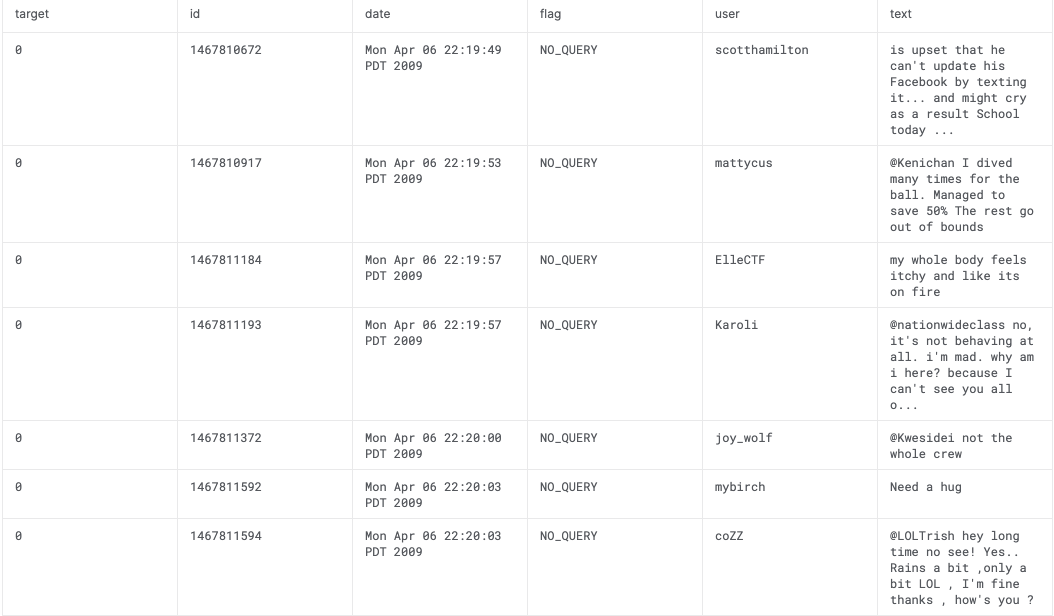
\includegraphics[scale=0.32]{twitter_overview.png}
    \caption{Overview of the Twitter dataset.}
    \label{fig:TWITTER_OVERVIEW}
\end{figure}

We noticed that users tend to make mistakes when posting new tweets either because of typos or replacement of english words with abbreviations or idiomatical terms (e.g. slang or internet jargon).
Therefore, we chose to perform major treatments on our data and tried to correct these errors in order to enhance the quality of our corpus (e.g. replace duplicated characters, 'hellooo' becomes 'helloo' and 'tooo much' becomes 'too much').

We decided to apply lemmatization and tokenization, which are common operations in NLP tasks, on our dataset, and in order to do that we relied on the spaCy pipeline ~\cite{startups:spaCy} because of its efficiency and nowadays many companies that deal with natural language processing have chosen to use it~\cite{data:companies_using_spacy}.

While it is common to tokenize sentences into words before passing them to a model, we thought it would be interesting to use lemmas instead of the original words since different variations of the original lemma have the same meaning (e.g. 'be', 'been' and 'am' refer to the same concept) and models should benefit from this process since they will have the chance to see multiple times the same lemma in different contexts.

Moreover, we managed to filter out from our corpus those common words that do not contribute to adding meaning to our sentences: the so called stopwords.
There is a plethora of valid collections of stop-words available on the web (e.g. NLTK~\cite{startups:nltk}, Gensim~\cite{startups:gensim}) and we decided to use those offered by spaCy.
%Although stopwords removal is something very common in many NLP tasks, we later discovered that there exist different categories of stopwords and some of them may be more relevant for our task.
%Along these lines, we experimentally crafted a set of stopwords that allowed us to get better results. Please refer to the next subsection for the relative discussion and the benchmarks.\\

%However, the preprocessing phase was not something that was specifically designed for the Twitter dataset, and we applied it to all the datasets we compared with (e.g. IMDb~\cite{data:imdb}) when necessary (we used other datasets to perfom some unusual tests, which will be discussed in some sections).

\subsection*{Effects of preprocessing}

At first, we expected this process to lead to good results since it simplifies the problem by removing a possibly long list of words whose presence can be neglected, but we had to change our mind about that.

Here in figure \ref{fig:PREPROCESSING_ROC} we can see some interesting results when testing our intuition on data preprocessing either for the multivariate Bernoulli or the multinomial na\"ive Bayes with word embeddings. 
Nevertheless, if we observe these ROC curves we discover some unexpected results: both the models achieved the best results when trained on non-preprocessed data.
%\clearpage


\begin{figure}[h!t]
    \centering
    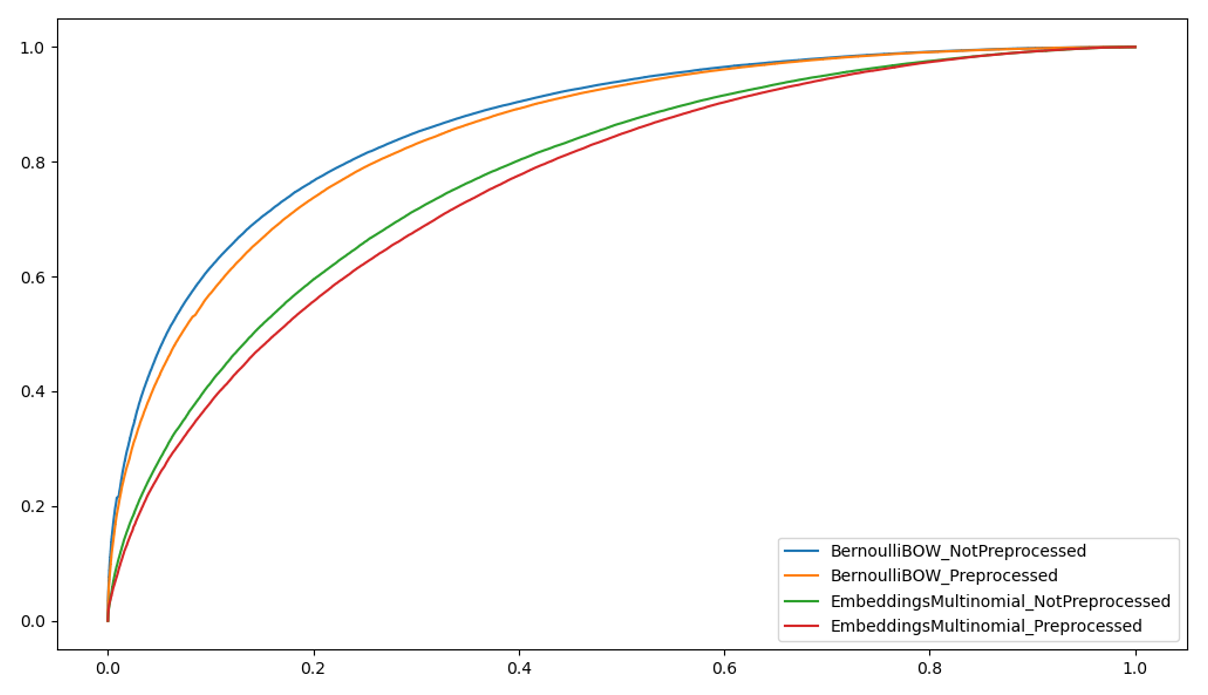
\includegraphics[width=11cm]{../experiments/plots/preprocessing.png}
    \caption{ROC curve with 80\% training and 20\% test.}
    \label{fig:PREPROCESSING_ROC}
\end{figure}


We struggled to understand why and we found two principal causes.
First, lemmatization is not always a good idea and in some cases using the original words instead of their lemma is the best choice.
More generally, this is a strong text manipulation technique and common sense tells us that if it does not allow us to gain a significant performance gain we should avoid it ~\cite{data:lemmatization_tips}. 
Second, it is not always a good idea to remove stopwords especially if the stopwords come from a general dictionary, in fact some words considered stopwords in a context might be useful words in another context. 
Using the spaCy stopwords the performance of our model decreased, instead using an ad-hoc set of stopwords (which contained only a few words such as articles and pronouns) we got some slightly better results compared to the case where no preprocessing at all is done.

%In particular, performing some ad-hoc stopwords removal, we managed to get even slightly better results compared to the case where no preprocessing at all is done. This confirms the intuition that not all stopwords are equal and there exist some stopwords that are more significant than others.

\begin{table}[h!t]
    \centering
    \caption{Comparing the results of preprocessing on our Bernoulli model. We randomly splitted the dataset in 80\% training set, 20\% test set.}
    \label{tab:stopwords}
    \begin{tabular}{c|c}
        \hline
        Preprocessing & Accuracy \\
        \hline 
        complete (spaCy pipeline) & 0.7690 \\ 
        none & 0.7828 \\ 
        ad-hoc stopwords removal & 0.7834 \\ 
        \hline
    \end{tabular}
\end{table}
